\section{AXI UART}

A universal asynchronous receiver transmitter (UART) is a computer hardware device for asynchronous serial communication in which the data format and transmission speeds are configurable. The electric signaling levels and methods are handled by a driver circuit external to the UART. Astrome has used multiple AXI UART IPs from Xilinx as UARTs for debugging and inter-communication between the device. The LogiCORE IP AXI Universal Asynchronous Receiver Transmitter (UART) Lite interface connects to the Advanced Microcontroller Bus Architecture (AMBA) specification\textquotesingle s Advanced eXtensible Interface (AXI) and provides the controller interface for asynchronous serial data transfer. This soft LogiCORE IP core is designed to interface with the AXI4-Lite protocol. The internals of AXI UART IP is shown in \figref{UART}.

\begin{figure}[H]
\begin{center}
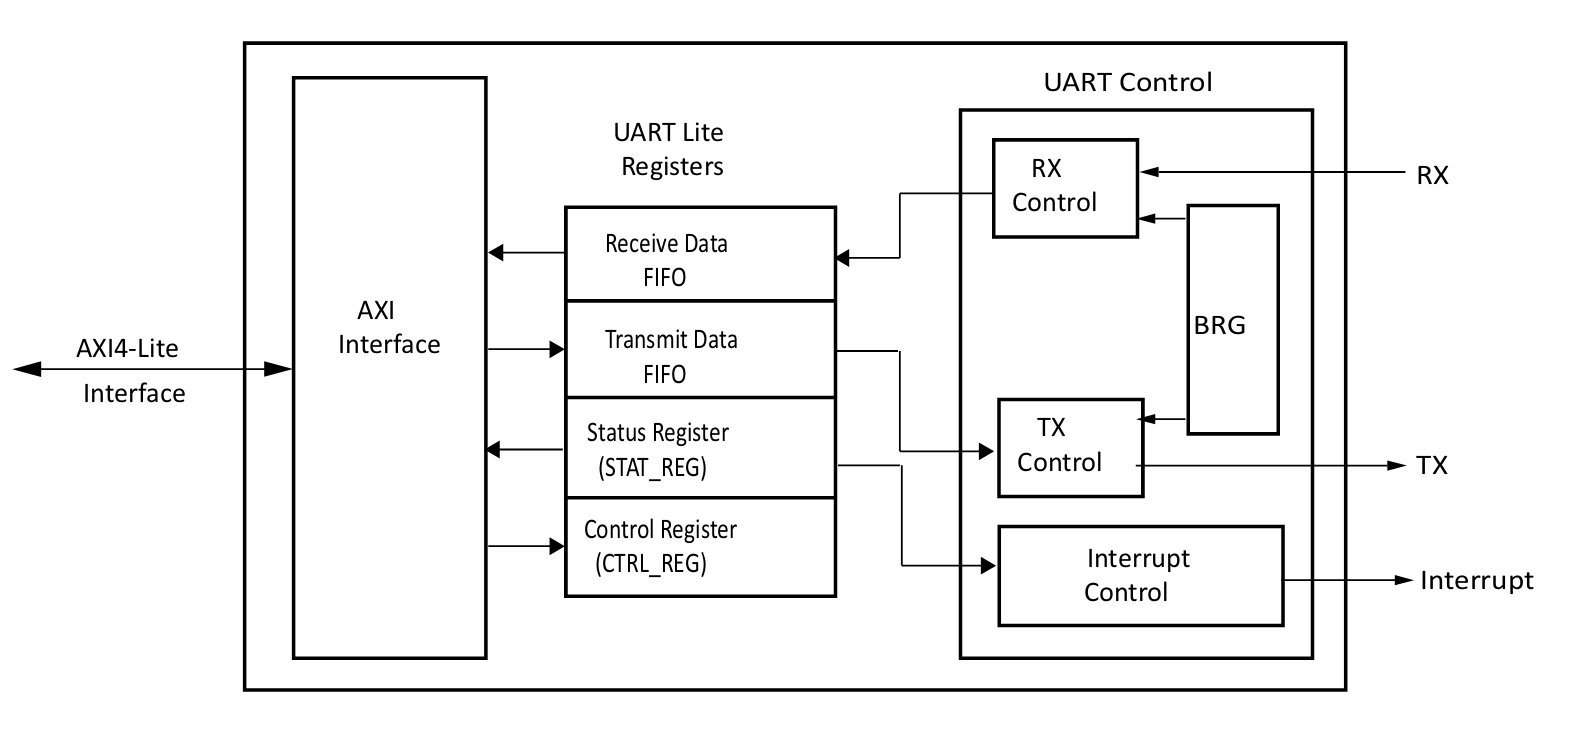
\includegraphics[width=\textwidth]{images/UART.png}
\caption{Internal block diagram of AXI UART IP}
\label{UART}
\end{center}
\end{figure}